%!TEX root=thesis.tex
%This is the draft literature review. 

%!TEX ROOT = thesis.tex


\chapter{Background Studies}
\label{section:litreview}

In this chapter, related theoretical background concepts are first introduced. Then, the related works are discussed in two main portions: 
\begin{enumerate}
    \item Existing methodology and techniques used for semantics extraction
    \item Recent methodology and techniques used for semantic retrieval.
\end{enumerate}



\section{Related Theoretical Background Concepts}
\label{subsec:relatedConcepts}

Before diving deeper into the nitty-gritty of the proposed framework, fundamental understanding towards related theoretical background concepts used in this work is discussed. As this work covers a rather broad spectrum of different concepts, a general understanding towards these concepts would provide some degree of clarity towards the topic at hand. This section briefly describes the fundamental of the following concepts: i) Quantization, ii) Distance Measure, iii) Human Visual System, \& iv) colour Model and colour Terms. 


\subsection{Quantization}

The use of quantization in the mathematical and digital signal processing field is not a new concept. Digital signal processors are limited by natural boundaries such as hardware limitations, and are only able to compute and perform arithmetic operations within a limited range \cite{spors_2018}. The use of quantization refers to the process of mapping and projecting a set of large values which are often continuous or analog in nature into a set of discrete and finite values. 

\begin{figure}[hbt!]\centering
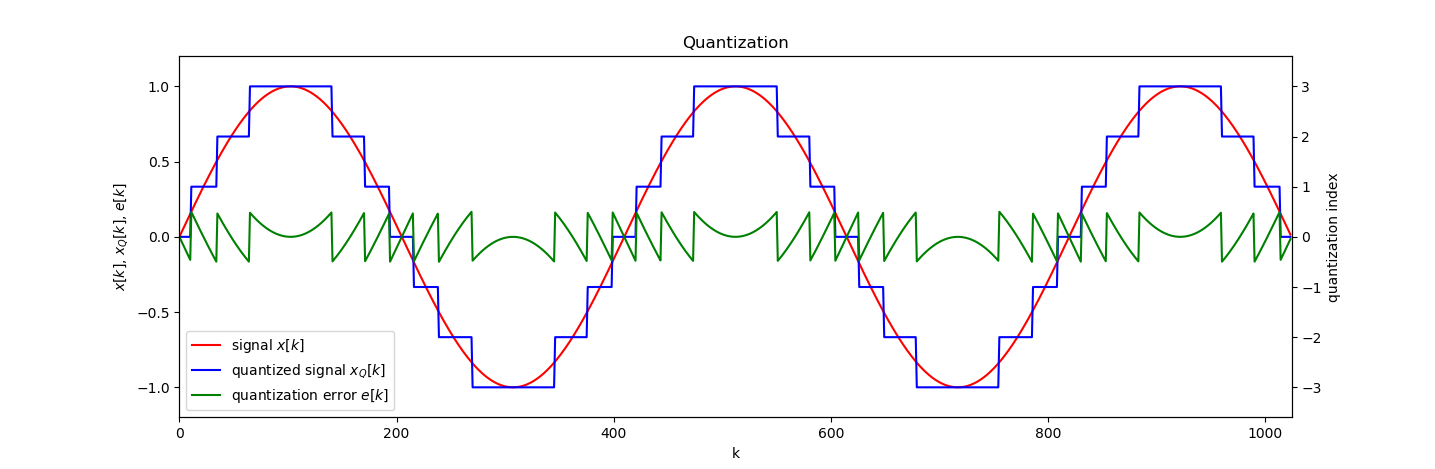
\includegraphics[width=\textwidth]{image/general/quantization.png}
\caption{Quantization}
\label{fig:quantize}
\end{figure}


The use of quantization enables reduction in memory usage (compression) as well as the reduction of computational cost, hence, leading to faster processing speed. However, since the quantization process is a many-to-few mapping operation, the operation is considered irreversible without prior knowledge of the loss. Nevertheless, the output discrete signal can closely resemble the continuous input signal depending on the number of quantization level used.
\begin{equation}\centering
\label{eq:quantization}
x_Q[k] = g( \mspace{3mu}\lfloor \mspace{3mu}f(x[k]) \mspace{3mu}\rfloor\mspace{3mu})
\end{equation} 
\vspace{-3em}
\begin{equation}\centering
\label{eq:quantizationerror}
e[k] = x_Q[k] - x[k]
\end{equation}
In order to expound on the quantization process, a mathematical model of this process can be formulated as such. Consider a continuous signal $x[k]$ whose quantized signal, $x_Q[k]$, is desired (see Equation \ref{eq:quantization}). The functions $f (\mspace{3mu} \cdot  \mspace{3mu})$ \& $g (\mspace{3mu} \cdot  \mspace{3mu})$ can be thought of as a real-value mapping function while the $\lfloor \mspace{3mu} \cdot  \mspace{3mu} \rfloor$ represents a rounding function. The $f (\mspace{3mu} \cdot  \mspace{3mu})$ function is used to convert real-world values into a digital signal, while $g (\mspace{3mu} \cdot  \mspace{3mu})$ is used to map the digital signal into a quantized signal. As previously mention, this process is considered irreversible with prior knowledge of the loss, in this case, the quantization error, $e[k]$, can be computed as Equation \ref{eq:quantizationerror}. Figure \ref{fig:quantize} illustrates a quantization process where the red signal ($x[k]$) represents the real-world continuous signal, the blue signal ($x_Q[k]$) refers to the quantized signal while the green signal ($e[k]$) represents the error due to quantization process.

In order to leverage on this concept, in this work, the quantization technique was extended further into a three dimensional space. As video data can be represented in a 3D space, the quantization process was used to quantize the continuous video data into a set of discrete and finite values. These discrete and finite values can ease the calculation and manipulation of data. As colour space can also be represented using a 3D space, this concept was adapted and applied here to quantize the colour space into colour terms (See Section \ref{section:colourterm}).



\subsection{Distance Measure}
\label{section:distancemeasures}

The use of distance measure is another recurring key concept in the proposed method. Given that distance measures are commonly used in computer science as well as the mathematics field, there are numerous metrics suggested by different authors which are applicable and useful in different scenarios. In essence, distance measure is used to compute the difference between targets. On the flip side, the difference can also be thought of as the similarity between these targets.

\begin{figure}[hbt!]\centering
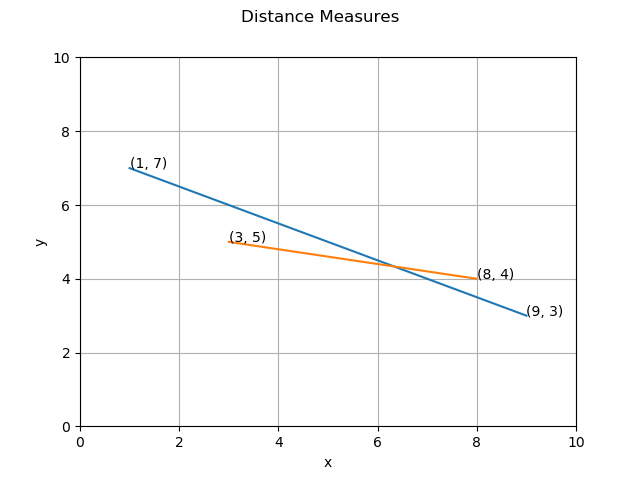
\includegraphics[width=.7\textwidth]{image/general/distance.png}
\caption{Example of Distance Measure}
\label{fig:distanceMeasure}
\end{figure}

To further accentuate on the concept of distance measure in this work, a simple example of how distance metrics can be applied in the proposed method is illustrated using Figure \ref{fig:distanceMeasure} with two plotted lines. In order to simplify the research problem, these lines can be thought of as vehicle trajectories captured over time that is flatten unto a 2D plot. Using the available data, the distance between two trajectories can be measured and used to signify the dissimilarity between them. This distance measure can also be used to identify trajectories with high resemblance. 

\begin{figure}[hbt!]\centering
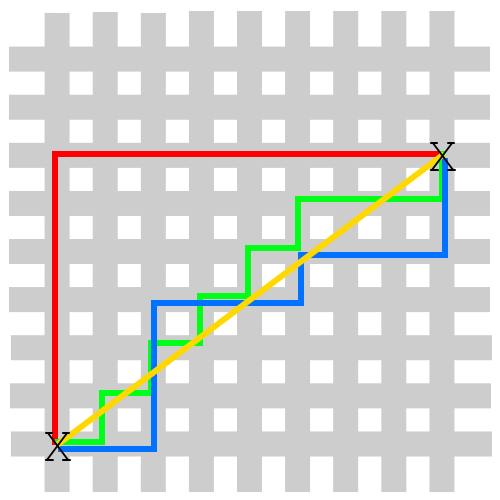
\includegraphics[width=.5\textwidth]{image/lit/manhattan.png}
\caption[Comparison between Manhattan Distance vs. Euclidean Distance]{With the assumption that each block has a equal distance of 1. Using Manhattan Distance, regardless of the path taken, the distance for the red, green and blue lines has the length of $14$. These 3 paths, while different, still takes on the shortest distance from one end to the other. However, when computing using Euclidean Distance, the distance is measured to be $\sqrt{8^2+6^2} = 10$. Euclidean Distance only produces $1$ unique solution while Manhattan Distance may produce more than one solution.}
\label{fig:manhattan}
\end{figure}


However, as different distance measure metrics are suitable for different scenarios, a good distance measure is an essential for comparing a significantly extensive set of vehicle trajectories during the retrieval process of a car park scene. This concept of distance measure was further extended into a multi-dimensional space such as the colours space, where the similarity between two or more colours were measured using different distance metrics to evaluate the performance of each metric. Table \ref{table:distance} lists out several distance measure which are commonly used along with the pros and cons of each while Figure \ref{fig:manhattan} shows the contrast between Euclidean and Manhattan distance.

\begin{table}[!ht]
\resizebox{\textwidth}{!}{
\begin{tabular}{|l|l|l|}
\hline
\textbf{Distance Measure} & \textbf{Pros} & \textbf{Cons} \\ \hline
Euclidean Distance & \begin{tabular}[c]{@{}l@{}}Simple, Fast,\\ Commonly used,\\ Able to work on n-Dimension data\end{tabular} & \begin{tabular}[c]{@{}l@{}}Vector order dependent,\\ Requires same length vectors\end{tabular} \\ \hline
Manhattan Distance & \begin{tabular}[c]{@{}l@{}}Reflection invariant,\\ Translation invariant,\\ Produces same result,\\ Able to work on n-Dimension data\end{tabular} & \begin{tabular}[c]{@{}l@{}}Requires same length vectors,\\ Does not have a unique solution\end{tabular} \\ \hline
Chamfer Distance & \begin{tabular}[c]{@{}l@{}}Able to work with \\ vectors of different length,\\ Vector order invariant, \\ Minimizes the difference \\ between vectors,\\ Able to work on n-Dimension data\end{tabular} & \begin{tabular}[c]{@{}l@{}}Higher computational cost,\\ Alternative matches may \\ receive equal distance\end{tabular} \\ \hline
Hamming Distance & \begin{tabular}[c]{@{}l@{}}Ensure similarity between vectors,\\ Able to work on n-Dimension data\end{tabular} & \begin{tabular}[c]{@{}l@{}}Vector order dependent,\\ Requires same length vectors\end{tabular} \\ \hline
\end{tabular}%
}
\caption{List of several distance measures along with their pros and cons}
\label{table:distance}
\end{table}




\subsection{Human Visual System}
\label{section:eyes}
The human eyes are visual system organs, responsible of receiving and processing visual information. Figure \ref{fig:eyes} shows a rough anatomy of the human eye. Within the eye, rods and cones are light-sensitive cells, found on the retina which are in charge of vision. Both of these cells plays a different role, rods cells are not able to perceive colour information, hence, they are known to be responsible for determining the lighting condition. On the other hand, cones cells are responsible for the reception of colour information. As human retina contains approximately 120 million rods and 6 million cones, the eyes are more sensitive toward lighting conditions. The sheer number of rods also enables humans to see in low-light achromatic vision.   


\begin{figure}[hbt!]\centering
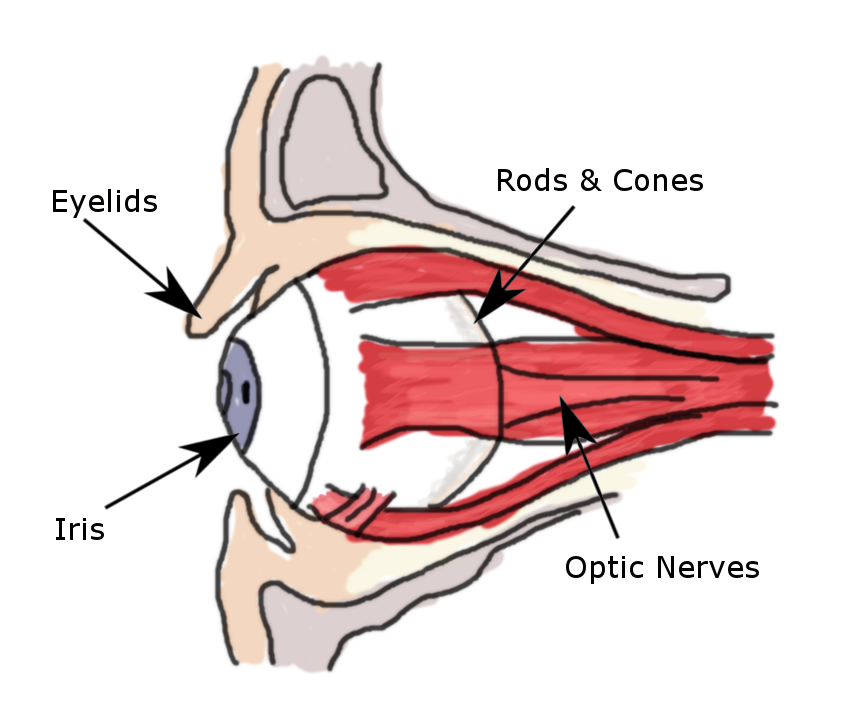
\includegraphics[width=.5\textwidth]{image/lit/rodsandconscolored.png}
\caption[Human Eye Anatomy]{Human Eye Anatomy. Rods and cones cells are responsible over human vision. When these cells on the retina are stimulated, signals are sent to the brain via the optic nerves. The brain would then processes these signals to provide vision for humans.}
\label{fig:eyes}
\end{figure}

Anatomically, there are three types of cones in the human retina, each of which are responsible over the receptiveness of colours in a particular type of wavelength. These wavelengths can be classified into three main categories: Short wavelengths light, Medium  wavelengths light and Long wavelengths light (See Figure \ref{fig:visibleSpectrum} \cite{eyespectrum}). colours are perceived from the combination of stimuli to these rods and cones cells and responses from brain. When stimulated, these cells fires electrical signals to the optic nerves fibres that communicates with the brain. However, as the number of cones cells in the retina varies for each person, the colour perception of everyone would differ in a way or another. 


\begin{figure}[hbt!]\centering
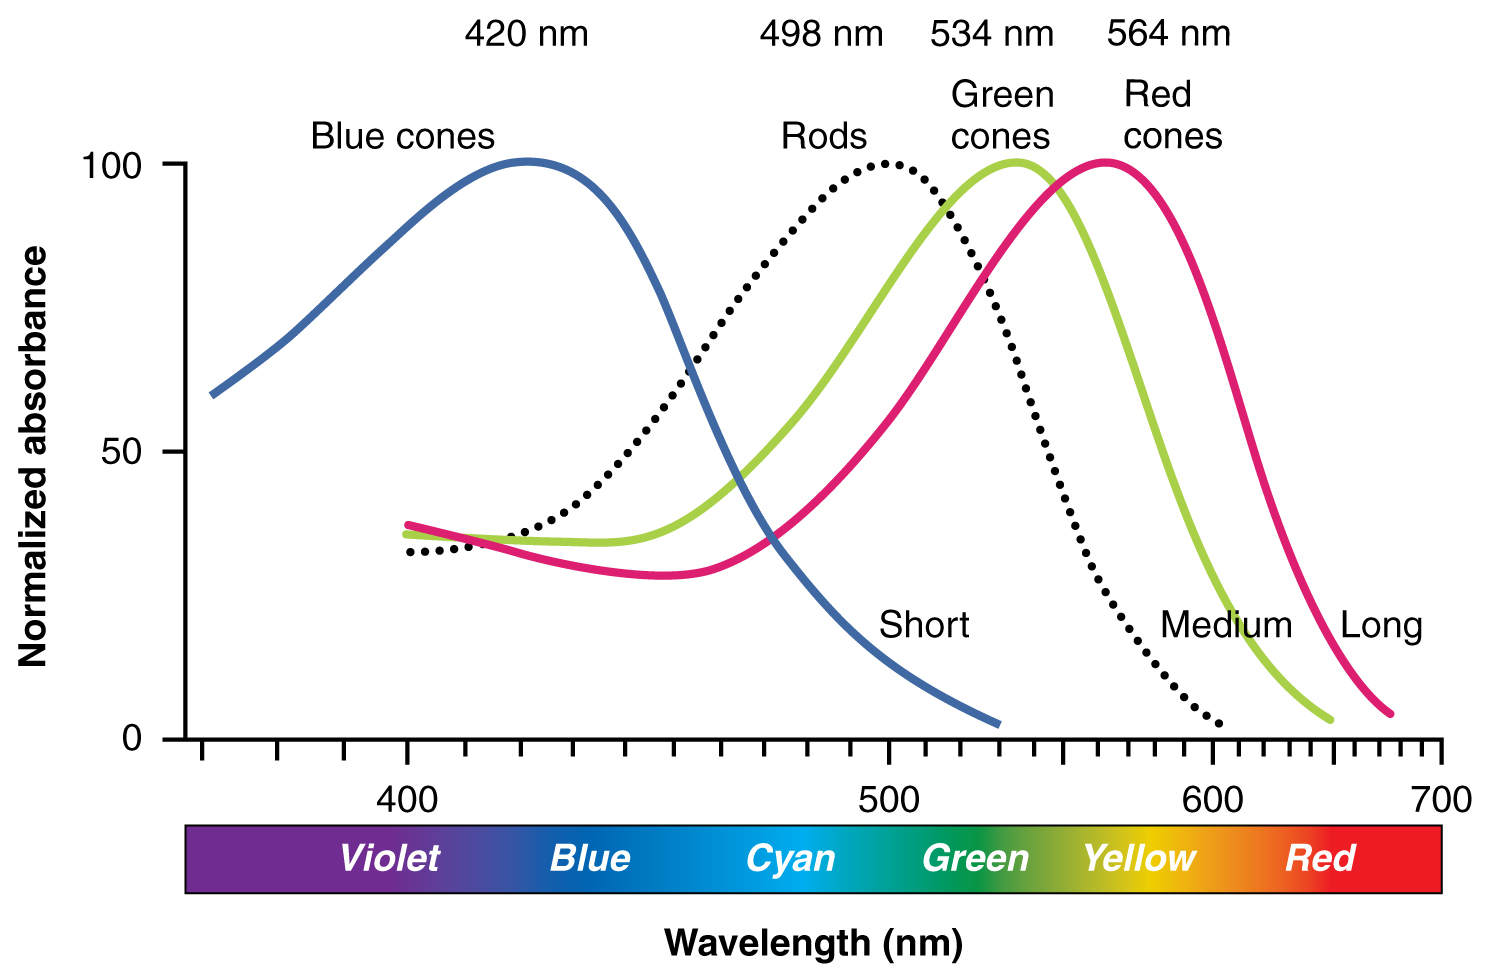
\includegraphics[width=.7\textwidth]{image/lit/ColorSensitivity.jpg}
\caption[Normalised human photo-receptor absorbency rate for different wavelength lights]{Normalised human photo-receptor (cons \& rods) absorbency rate for different wavelengths of light. 'Blue' cones, approximately 420-440 nm, are short wavelengths light; 'Green' cones, approximately 534-545 nm, are medium wavelengths light; and, 'Red' cones, approximately 564-580 nm, are long wavelength lights }
\label{fig:visibleSpectrum}
\end{figure}




\subsection{Colour Model, Systems and Terms}
\label{section:colourterm}

In order to represent colours in tuples of number, colour models were designed. In essence, it can be thought of a quantization process of converting a series of real-world continuous signal (colour wavelengths) into a set of finite tuples of numbers within a colour model. 
With the ability to quantize these wavelengths into sets of finite tuples, the colours can be digitised and used for further processing.


\subsubsection{Colour Models}
From the previous section, the humans' visual system was explored. From there, it is learnt that the cones cells in the retina are strongly receptive towards stimuli of 'Red', 'Green' and 'Blue' wavelengths. Given the solid theory behind human perception of colours, the RGB colour model was designed. This colour model is commonly used to represent and display images in digital systems. 

As an example, the RGB colour space is an additive colour model, each of the components (R, G, B) are added together to produce the final colour. Typically each of these components are represented using 8 bits, hence, 256 possibilities for each component with a total of $256 \times 256 \times 256 = 16M$ colour combinations in total. As this is an additive model, 'Black' colour is  represented using $(0, 0, 0)$, while 'White' using $(255, 255, 255)$. Figure \ref{fig:rgb} represents this colour model.

\begin{figure}[hbt!]\centering
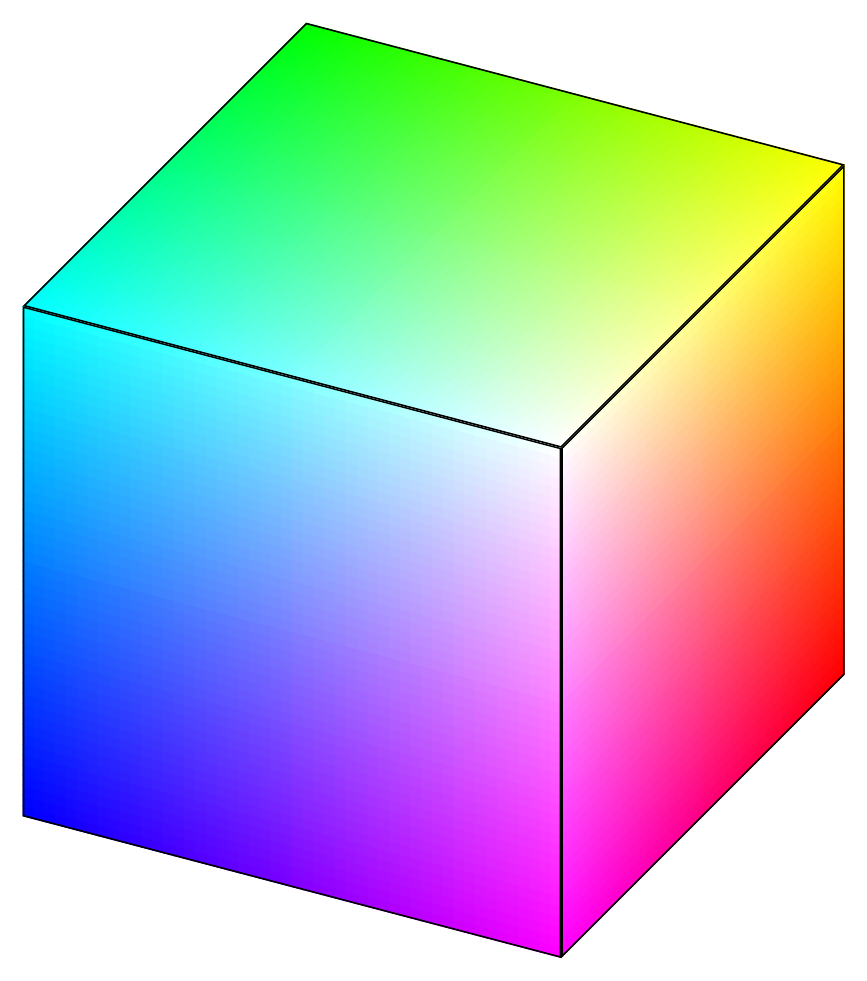
\includegraphics[width=.4\textwidth]{image/lit/rgbcolor.jpg}
\caption{RGB colour Model}
\label{fig:rgb}
\end{figure}


\subsubsection{Munsell Colour System}
\label{section:munsellcs}
colour terms - such as "Red", "Green" or "Blue", are commonly derived from the Munsell colour system which was created in the early 20th century by Professor Albert H. Munsell. The Munsell colour System was designed to organise colours similar to how the human's eye sees - which is, by organising colours according to their hues, followed by the chromatic range and the brightness values in a perceptually uniform manner. 

For each horizontal circle on the Munsell colour System, the hues can be divided into 5 principle hues which are Red, Yellow, Green, Blue, and Purple. This setup allows another 5 intermediate hues in between each principle hues, for example: Green-Blue hue, Purple-Red hue. 
Figure \ref{fig:munsell}(a) illustrates the Munsell colour System while Figure \ref{fig:munsell}(b) illustrates the property of the chroma and value scale available on the Munsell colour system, for example, a hue at 2.5 Yellow-Red (YR) has a maximum chroma value which differs along the value axis. 



\begin{figure}[!htb]
  \centering
  \resizebox{\textwidth}{!}{
\begin{tabular}{cc}
 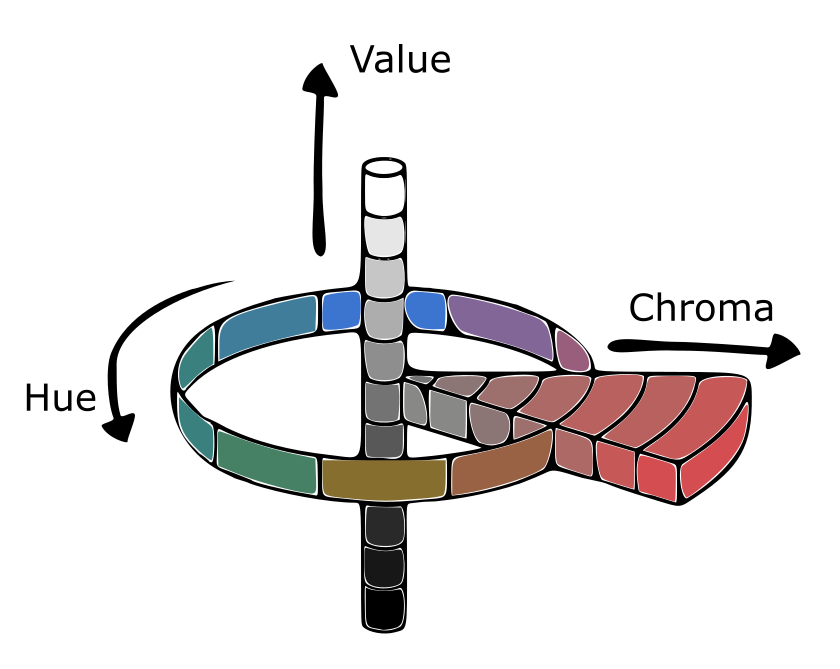
\includegraphics[width=0.4\linewidth]{image/general/munsell.png}  &
 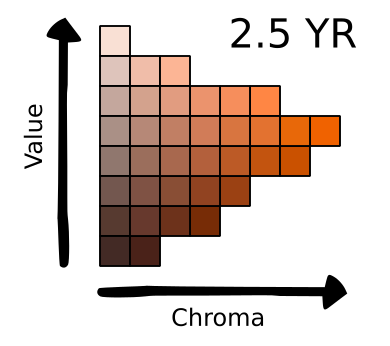
\includegraphics[width=0.4\linewidth]{image/general/25YR.png}\\
 (a) Munsell colour System &
(b) Hue at 2.5YR with various Chroma and Value\\
\end{tabular}}
\caption{Munsell colour System} \label{fig:munsell}
\end{figure}



\subsubsection{Colour Terms}

While the basic idea of colours seems to be a relatively simple idea for humans, machines on the other hand, do not understand the concept of colours. Modern computers generally represents colour values using the Red-Green-Blue (RGB) values for most applications. Despite its frequent usage, it is difficult for humans to visualise a particular colour when presented with three RGB values as these values does not directly translate the intuitive nature of a particular colour. Along with that, it is also very difficult to visualise the difference between two colours using the RGB values only. 

Table \ref{table:allcolourterms} lists several popular web colour dictionaries along with the number of colour terms as well as the publishing year. One notable property of these colour terms is the use of compound terms such as 'baby blue', 'dark red', 'light purple' and 'very deep brown'. Along with that, in some colour dictionary, certain colours terms are duplicated for several tuples. Given the variety of colour dictionaries and the number of different colour terms, one of the targets in this work is to investigate and decide how many colour terms should be allocated to describe the vehicle colours. 

\begin{table}[hbt!]
\centering
\begin{tabular}{|c|c|c|}
\hline
\multicolumn{1}{|c|}{\textbf{Web Colour Dictionary}} & \multicolumn{1}{c|}{\textbf{Number of Colour Terms}} & \multicolumn{1}{c|}{\textbf{Year}} \\ \hline
x11 (R3)                                            & 631                                                 & 1988                               \\ \hline
HTML                                                & 140                                                 & Current                            \\ \hline
CSS                                                 & 148                                                 & Current                            \\ \hline
Crayola                                             & 248                                                 & Current                            \\ \hline
xkcd                                                & 954                                                 & 2010                               \\ \hline
\end{tabular}
\caption[Web Colour Dictionary and the corresponding number of colour terms]{Web Colour Dictionary and the corresponding number of colour terms}
\label{table:allcolourterms}
\end{table}

%https://people.csail.mit.edu/jaffer/colour/Dictionaries
% x11 colours: https://groups.google.com/forum/?fromgroups=#!topic/comp.windows.x/AYPozZhQxok
% https://www.crayola.com/explore-colours.aspx
%http://markkness.net/colourpy/colourPy.html










\section{Related Works}
\label{section:relatedworks}

The advancement of computer vision technologies enabled the development and integration of various solutions to tackle challenges in Intelligent Transportation Systems (ITS). As ITS is a big topic, there has been a substantial increase of research done on the various subdomains. With the amount of research done, instead of reinventing the wheel, existing frameworks were adopted and leveraged upon. Recent survey done by \cite{tian2017hierarchical} and \cite{chandran2017review} were studied to understand the general overview of the state of related works. The authors has summarised the challenges that are often found in an ITS setting that is implemented on a one-camera setup: 
\begin{enumerate}
    \item \textbf{Camera placement} affects the overall performance. 
    \item The \textbf{lighting condition} varies throughout the day. Supplemental lighting equipments can be used during the night, however, the visual range will be limited.
    \item Vehicles are often \textbf{occluded} in an ITS setting; often by pedestrians, bicycles, trees, and even buildings.
    \item \textbf{Vehicle pose} varies when turning or changing lanes.
    \item Vehicles comes in a \textbf{variety of shapes, sizes, and colour.}
    \item As \textbf{vehicles' size changes} as it pass through the camera's field of view. This variation in visual information affects the robustness of some detection models. 
\end{enumerate}
Along with that, \cite{tian2017hierarchical} has presented an overview of the general frameworks for ITSs with the aim of vehicle attribute extraction and behaviour understanding in Figure \ref{fig:ITSoverview}. 
As mentioned in Section \ref{subsec:scope}, the bounding box of each vehicles are assumed to be obtained prior to the semantic extraction task, related literature regarding the detection and tracking of vehicles will not be discussed. 
Instead, the rest of this section is expounded under two main categories: i) Objects Semantic Extraction, and ii) Object Semantic Retrieval. 


\begin{figure}[hbt!]\centering
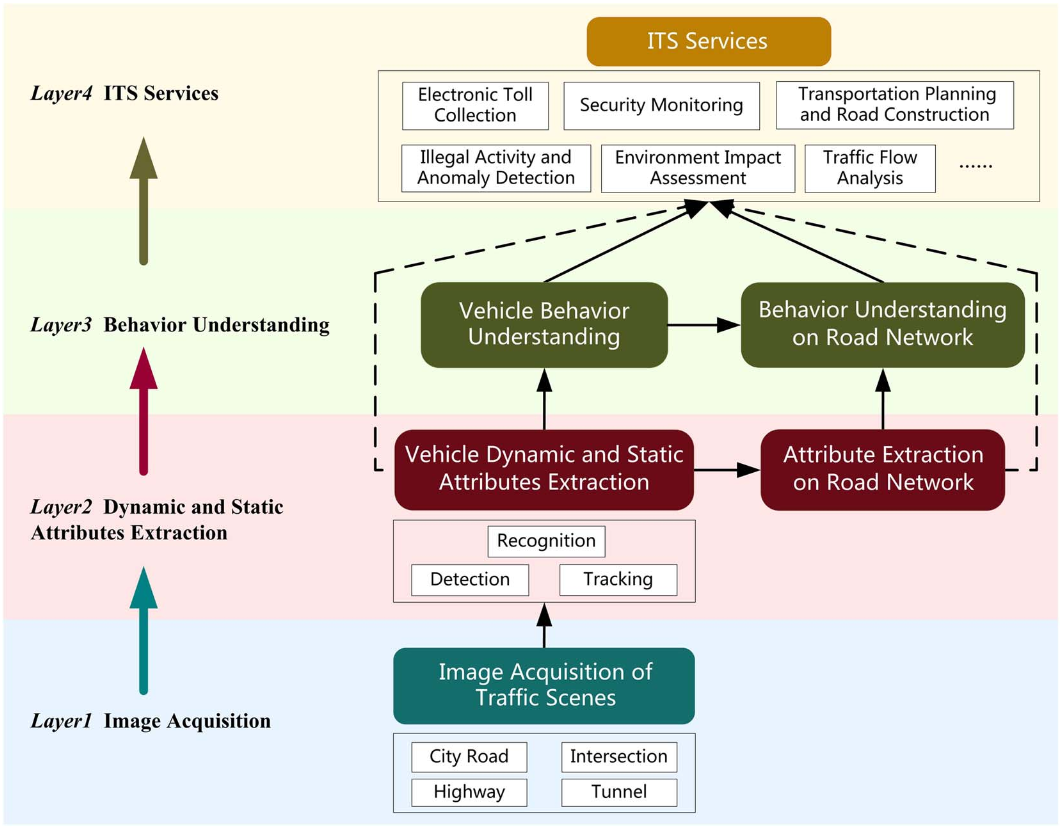
\includegraphics[width=.8\textwidth]{image/lit/ITS.png}
\caption[Overview of the General Frameworks for ITSs]{(From Bottom) Layer 1: The process of obtaining data via vision sensors. Layer 2: Attribute Extraction from data; this includes motion, trajectories, colours, shapes and etc. Layer 3: Analysis on vehicle behaviours from the extracted attributes to decide traffic status. Layer 4: Utilises information from Layer 3 to optimise various ITS services. Figure reproduced from~\citeA{tian2017hierarchical}}
\label{fig:ITSoverview}
\end{figure}




\subsection{Object Semantics Extraction}


The extraction of Vehicle colours is essential for a wide variety of applications in ITS such as crime prevention and security purposes. \cite{hsieh2015vehicle} noted that in an full-day surveillance scenario, the varying illumination as well as the camera viewpoint in an outdoor scene affected the classification of colours drastically. In that work, the vehicles are grouped into seven categories (Figure \ref{fig:sevenclasses}) via colour correction method. As the vehicle windows appear white due to the effects of specular highlights, the authors also proposed a window-removal task to increase the accuracy. This work also proposed the classification of vehicles into chromatic and achromatic classes, the final colour category is decided via Support Vector Machine (SVM). 

\begin{figure}[hbt!]\centering
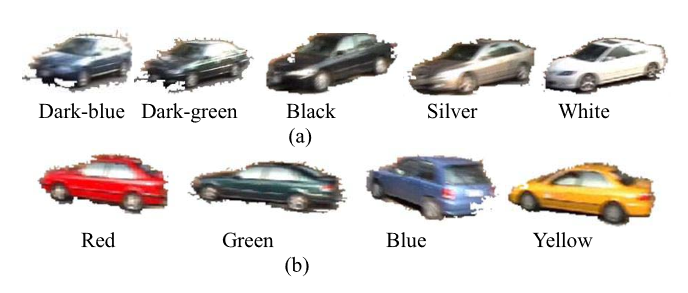
\includegraphics[width=.4\textwidth]{image/lit/carscolors.png}
\caption[Colour Appearance Categories of  Vehicle  Used  for  Colour Classification]{(a) Vehicles Classified as "Achromatic"; (b) Chromatic Vehicles. Reproduced from \cite{hsieh2015vehicle}.}
\label{fig:sevenclasses}
\end{figure}


.In[105]knearestneighborlikeclassifierwasusedtoclassifyvehiclecolorintosixgroups,eachofthemcontainssimilarcolorslikeblack,darkblueanddarkgray.HSVcolorspacewasusedin[106].Theyclassifyvehiclecolorintored,blue,black,whiteandyellowusing2-DhistogramofHandSchannelstogetherwithSVM.Multipleclassificationmethods(K-NN,ANNsandSVM)alongwithtworegionofinterestwereusedin[107]torecognizevehiclecolorina16colorspace.In[108]bagofwordtechniquewasusedtoselectregionofinterestforcolorrecognition






\subsection{Object Semantics Retrieval}

According to the survey by \cite{chandran2017review}, trajectory retrieval algorithms can be largely divided into two categories: i) String  Matching Algorithm, and ii) Sketch Matching Algorithm. String matching algorithms   




longest   common   subsequence   (LCSS)   algorithm complete  string-based  matching  trajectories  by  per-forming  a  frame-by-frame  analysis  directly  on  ob-jects’ coordinates. The  work  in  [3]  assumed a  query  by  example  me-chanism  according  to  presented  example  trajectory and  the  search  system  could  return  a  ranked  list  of most similar items in the data set by a string matching algorithm,  whereas  the  sketch-based  method  projects a trajectory on a  set ofbasic functions and matches it according to its low-level geometrical features.